\documentclass[runningheads]{llncs}

\usepackage[spanish]{babel}
	\selectlanguage{spanish}

\usepackage{graphicx}
	\graphicspath{{img}}

\title{Sistemas distribuidos en MMORPGs}

\author{Atanasio José Rubio Gil y María Sánchez Marcos}
\institute{Universidad de Granada, 18010 Granada, España}

\begin{document}
\maketitle

\begin{abstract}
Una de las aplicaciones de los sistemas distribuidos son los videojuegos multijugador masivos.
Estos servicios plantean retos a los desarrolladores a la hora de diseñar las interacciones, pues deben tener en cuenta que los jugadores se van a conectar entre ellos y con el servidor para interactuar y que sus acciones repercuten en la experiencia del resto de jugadores, por lo que deben poner mucho esmero en crear sistemas que funcionen correctamente y de forma segura para todos los participantes.
Cada juego elige sus propios métodos de gestionar las conexiones y organizar a los jugadores, con sus particularidades y arquitecturas propias, de forma que se ajusten al tipo de jugabilidad que presentan y sus necesidades de interacción entre los usuarios y las de éstos con el entorno.

\keywords{MMORPG \and Servidor \and Sistemas distribuidos.}
\end{abstract}

\section{Introducción}

Los videojuegos de rol multijugador masivos en línea, globalmente conocidos como \textbf{MMORPG} por sus siglas en inglés (\textit{Massively Multiplayer Online Role-Playing Game}) son videojuegos que permiten a miles de jugadores introducirse en un mundo virtual de manera simultánea a través de internet e interactuar con él y otros jugadores asumiendo un papel dentro de dicho mundo.
Este género de videojuegos es especialmente interesante en cuanto a lo que nos atañe, debido a que el límite de jugadores que estos permiten dependen exclusivamente de las características del juego y de la capacidad de su infraestructura de servidores.
Muchos MMORPGs tienen incluso múltiples servidores distribuidos según las regiones para permitir así un número de jugadores muchísimo mayor.

Independientemente del reto que pueda suponer tal cantidad de jugadores, también existen otras problemáticas que deben resolverse.
Debemos tener en cuenta que no solo sus jugadores interactúan entre ellos, sino que el entorno es afectado por los jugadores, es decir, una acción que haya sido llevada a cabo en un lugar del mundo, puede tener repercusiones para los jugadores de otro lugar totalmente diferente.
Se trata de un ambiente dinámico, en constante cambio y con repercusiones a nivel global.

Aparte de problemas más asociados al diseño narrativo y de niveles que puede tener cualquier juego (calidad de la historia, construcción del universo, capacidad de captar la atención de los jugadores en las misiones, personajes carismáticos\ldots), los MMORPGS se enfrentan a problemas producidos por la necesidad de conexión constante entre los jugadores.

Algunas de las cuestiones que se plantean los desarrolladores a la hora de diseñar el sistema de conexión son:~\cite{mmg_love}

\begin{itemize}
	\item
		¿TCP o UDP\@?
	\item
		¿Consistencia y escalabilidad?
	\item
		¿Peer to peer o cliente-servidor?
	\item
		¿Baja latencia o confiabilidad?
	\item
		¿Cómo controlar la congestión?
	\item
		¿Compatibilidad para el soporte de diferentes plataformas?
	\item
		¿Cómo controlar la seguridad (\textit{hashing} de mensajes, encriptación, \textit{anti-spoofing}\ldots)?
\end{itemize}

En este documento trabajaremos sobre algunos de estos temas y estudiaremos algunos de estos videojuegos para ilustrar lo estudiado.

\section{Consistencia}

El objetivo principal de un juego multijugador es ofrecer a cada jugador una vista consistente y constante del mundo en el que se halla.
Para ello, los clientes deben estar recibiendo continuamente actualizaciones de los cambios que ocurren en el mundo.

\subsubsection{El problema del cofre}~\cite{dge_mmosg}
Supongamos que existe un grupo de jugadores que entra en una mazmorra y consigue un cofre.
En el cofre hay probabilidades de que al abrirlo aparezca una bomba o una moneda.
En primer lugar, una vez uno haya abierto el cofre, todos deben ver el mismo objeto, no deberían poder algunos una bomba y otros una moneda.
Pero no solo eso, deben verlo todos en el mismo instante para tener las mismas oportunidades de cogerlo, aunque esto también puede depender de la conexión de los jugadores.

En el momento en el que intenten coger la moneda, ¿quién se la lleva? Una vez se lo lleve uno, los demás jugadores no deben poder verla, ni cogerla.
Esto se resolverá con un sistema de autoridades en los objetos del mundo.
De esta manera, cuando dos jugadores decidan coger la moneda, ambos mandarán una petición a la autoridad y solo uno de ellos obtendrá el permiso para tomarla.
Obviamente, muchas peticiones suponen una sobrecarga  en las interacciones que requieren una autorización para que el juego pueda continuar.

Además, debemos diferenciar que esta mazmorra estará aislada del resto del mundo y solo será accedida por este grupo.
Esto se llama \textit{gameplay} localizado y facilita la consistencia local.

\section{Latencia}

La latencia es el tiempo que supone la comunicación de un mensaje entre emisor y receptor.
Es un aspecto muy importante ya que una mala latencia puede suponer que el jugador no tenga una sensación de juego en tiempo real.

\pagebreak

Podemos definir la latencia de dos maneras:~\cite{dge_mmosg}

\begin{itemize}
	\item\textbf{Latencia unilateral:}
		Tiempo que toma un paquete en llegar del emisor al receptor.
	\item\textbf{Latencia de ida y vuelta:}
		Es el tiempo que toma el paquete en llegar al receptor y recibir una respuesta de vuelta.
\end{itemize}

\subsubsection{Protocolos de comunicación}

La comunicación de mensajes sigue diferentes protocolos, no se rige únicamente por uno.
TCP asegura la llegada de los paquetes, sin embargo añade una sobrecarga extra en cuanto a esfuerzo y esto puede hacer que la latencia aumente.
Por tanto, también se intercalan envíos de paquetes con protocolo UDP, de manera que el mensaje, aunque no asegura del todo la integridad del paquete, es mucho más rápido.
Hay juegos que exigen una latencia muy baja, por ello hacen exclusivamente envío de mensajes con UDP\@.

Enviar el estado de un juego entero por UDP es muy pesado y poco seguro pues, como hemos dicho, no garantiza la seguridad del paquete, por ello se utiliza el Delta-Encoding.

\subsubsection{Delta-Encoding}

El Delta-Encoding es un tipo de cifrado que consiste en evaluar dos estados del juego y enviar la diferencia entre ambos.
De esta manera, el envío es muy ligero.
Además, a pesar de que puede parecer un problema que los paquetes se pierdan, al usar el Delta-Encoding junto con un protocolo de verificación de llegada este problema se soluciona.

\begin{figure}[ht!]
\begin{center}
	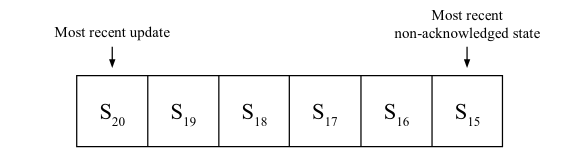
\includegraphics[scale=0.6]{delta.png}
\end{center}
\caption{Transición lineal entre dos estados usando Delta-Encoding}
\end{figure}

\section{Escalabilidad}

La escalabilidad en el ámbito de los sistemas distribuidos es la capacidad de usar más o menos recursos dependiendo de la carga de trabajo exigida.
En un MMO, la carga de trabajo suele ser dependiente del número de jugadores que haya y los recursos son los servidores o Hardwares.

Es necesario crear la estructura de servidores lo más escalable posible para poder soportar el creciente número de jugadores en un MMO~\cite{dge_mmosg}.
Esta enorme cantidad de personas jugando simultáneamente, aumentará la carga de trabajo del servidor y a menos que el sistema de servidores sea escalable y funcional, los jugadores experimentarán un gran aumento de la latencia.

Realmente, es un problema relativamente fácil de solucionar.
Es necesario aumentar el número de servidores o ponerlos más potentes, esto hará que la carga de trabajo se distribuya mejor.
Sin embargo, tenemos que tener en mente que si esto quiere realizarse, el arquitecto de redes debe diseñar la red de servidores con la escalabilidad y elasticidad en mente, para que el añadir nuevo hardware no sea un problema en el futuro y se consiga que el juego que se está diseñando tenga una vida útil mucho más larga.

Si una zona del mapa en concreto se llena de jugadores (crowding), que es un fenómeno muy usual en los MMO, puede ocurrir que la latencia aumente en un grado muy alto y las interacciones entre jugadores pueda ser molesta.
Esto es todo un desafío para los creadores de videojuegos.
Para solventar esta problemática, los MMO explotan la mecánica anteriormente mencionada del gameplay localizado, ya que de esta manera, se facilita lo consistencia local y se emplea la agrupación de servidores (server clustering) y equilibrio de carga (load-balancing) para conseguir una buena escalabilidad.

\section{Seguridad}

La seguridad es un gran problema en cualquier juego online, no solo en los MMOs.
Existen diversas formas en la que un jugador con conocimientos de informática/redes más o menos básicos pueden hacer trampas en el juego.
Fallas en el sistema de seguridad pueden arruinar la experiencia de juego para todos los demás jugadores.
Cuantos más archivos, datos y control se ofrezcan al cliente, más alta es la probabilidad de que un jugador identifique y haga uso de un agujero en la seguridad del sistema~\cite{datacomm}.

Todo el software instalado en la parte del cliente está expuesto a ataques y puede revelar información sobre la arquitectura del juego.
Los packet sniffers son programas que monitorizan y muestran los mensajes enviados y recibidos por la red y están disponibles para todos los usuarios.
Con ayuda de estos programas, un usuario con intenciones maliciosas puede modificar o bloquear paquetes antes de que se envíen desde el cliente.
Por lo tanto, se podría, por ejemplo, eliminar los paquetes que contienen acciones que no le convienen a esta esta persona.

Una de las soluciones a este problema, es la encriptación.
Desafortunadamente, la encriptación y la desencriptación consumen mucho tiempo y esfuerzo, esto hace que no siempre sea una práctica adecuada.

Otra solución puede ser otorgar a cada paquete un número de serie que el receptor comprobará antes de hacer uso de este paquete.
Si el número de secuencia de un paquete difiere del original, este será rechazado.
Con esta aproximación se puede descubrir el duplicado de paquetes y otras prácticas fraudulentas.
Para aumentar la seguridad, también se puede añadir un checksum a los datos transferidos, para que el servidor los compruebe y valide.

\section{Arquitecturas de servidores}

La práctica más común a la hora de gestionar los miles de jugadores de un videojuego multijugador masivo es distribuir la población alrededor de varios servidores o fragmentos o \textit{shards}, cada uno de los cuales se encarga de gestionar un subconjunto de los jugadores.
Este sistema es el preferido por muchos desarrolladores porque alivia el trabajo de gestionar un conjunto de jugadores demasiado grande interactuando con el entorno y entre ellos.

\subsection{Servidores regionales}

Uno de los enfoques más sencillos a la hora simplificar la estructura de la distribución de los servidores es dividir a los jugadores en servidores aislados entre sí, de forma que las interacciones se encuentren encapsuladas dentro de cada uno de los servidores.
De esta forma, los desarrolladores tienen la ventaja de que pueden localizar los servidores regionalmente, lo cual les evita la obligación de gestionar un abanico de tiempos de latencia tan amplio como ocurriría en servidores disponibles globalmente.
A pesar de que juegos como League of Legends adopten este enfoque más pragmático que técnico, jugadores de distintas regiones siguen pudiendo conectarse a regiones ajenas a la suya; sin embargo, lo deben hacer teniendo en cuenta que van a jugar con una latencia mucho mayor a la que jugarían si se conectaran al servidor de su región, pero se elimina implícitamente la responsabilidad de los desarrolladores de gestionar operaciones concurrentes con un rango de tiempos de latencia a nivel global.
Si el jugador experimenta un exceso de tiempo de sincronización, es responsabilidad suya.

\subsection{Otros modelos de distribución de los servidores}

\subsubsection{RuneScape}
Cabe destacar el caso del videojuego de la empresa sajona Jagex.
En RuneScape, los jugadores se dividen en servidores o \textit{mundos} divididos regionalmente, de forma que un jugador de California se conectará a un servidor estadounidense mientras que un jugador granadino podrá decidir conectarse a los servidores alemanes, holandeses o ingleses.
Sin embargo, la división regional de los servidores no es un factor determinante a la hora de gestionar la cuenta, como ocurre en otros juegos; los jugadores son libres de saltar (\textit{world hop}) entre todos los servidores distribuidos globalmente en cuestión de segundos sin necesidad de tener una cuenta distinta en ellos o sin siquiera volver a introducir los credenciales.
Este diseño presenta dos grandes ventajas para los desarrolladores y los jugadores.

Primero, los servidores pueden adoptar diferentes temáticas tanto implícitas como explícitas~\cite{osrs_servidores}.
Por ejemplo, si un servidor indica que es el apropiado para realizar una actividad en grupo, los jugadores acudirán a él para realizar esa actividad, de forma que la carga de jugadores congregados en diferentes actividades se disminuye y permite que jugadores que deseen jugar en dicha actividad en solitario o en un grupo reducido lo pueden hacer en el resto de servidores.
Explícitamente, un servidor puede programarse para permitir combate PVP (\textit{Player VS Player}), de forma que cualquier jugador puede atacar a otros jugadores a lo largo del territorio de juego~\cite{osrs_bh}, mientras que en el resto de servidores no se permite, congregando en él a los jugadores que prefieren este estilo de juego.

Por otro lado, los jugadores tienen la libertad de cambiar de servidor para participar en una actividad si el servidor en el que se encuentran no les parece adecuado.
Por ejemplo, si una cantera se abarrota de jugadores picando las piedras y agotando los recursos más rápido de lo que se renuevan, algunos de los jugadores presentes y los que vayan a comenzar la actividad pueden saltar a otro mundo para realizar la actividad con menos jugadores compitiendo.

\subsubsection{EVE Online}
Un sistema totalmente opuesto es el que utiliza CCP Games para gestionar el único servidor~\cite{eve_shard} que contiene toda la información de EVE Online, un videojuego multijugador masivo online en el que los jugadores controlan la economía y política de una galaxia y todos sus sistemas solares.
El enfoque de utilizar un único servidor les permite asegurarse de que todos los usuarios se concectan a la misma instancia, de forma que la comunidad no se encuentra fragmentada en diferentes regiones.

Kjartan Emilsson, desarrollador del videojuego, plantea que gran parte del reto de limitar la densidad de jugadores en una zona concreta del juego viene dada por la cantidad de contenido que los creadores son capaces de desarrollar: A mayor cantidad de contenido, más diversificación de los jugadores~\cite{inf_space}.
Sin embargo, esto acarrera costes de desarrollo que CCP Games ha evitado eliminando el contenido ``del videojuego'' y centrando el desarrollo en favorecer que los jugadores y sus interacciones sean la piedra angular de la interacción.
Con esta y muchas otras simplificaciones del sistema, los desarrolladores son capaces de afrontar el reto de gestionar toda la información del juego en un único servidor.

Arquitecturalmente, el juego divide sus conexiones en múltiples servidores \textit{proxy} distribuidos a lo largo del mundo que se conectan a servidores SOL con información local a los jugadores.
Estos servidores, a su vez, realizan llamadas de lectura/escritura constantes a la base de datos central, situada en Londres~\cite{eve_server}.
Para trabajar en concurrencia con su entorno, los servidores trabajan con las herramientas que ofrece el lenguaje Stackless Python~\cite{spython} y con unas directivas extrictas de trabajo con la base de datos central que les permiten realizar accesos no bloqueantes a la misma sin corromper los datos.

\begin{figure}[ht!]
	\begin{center}
		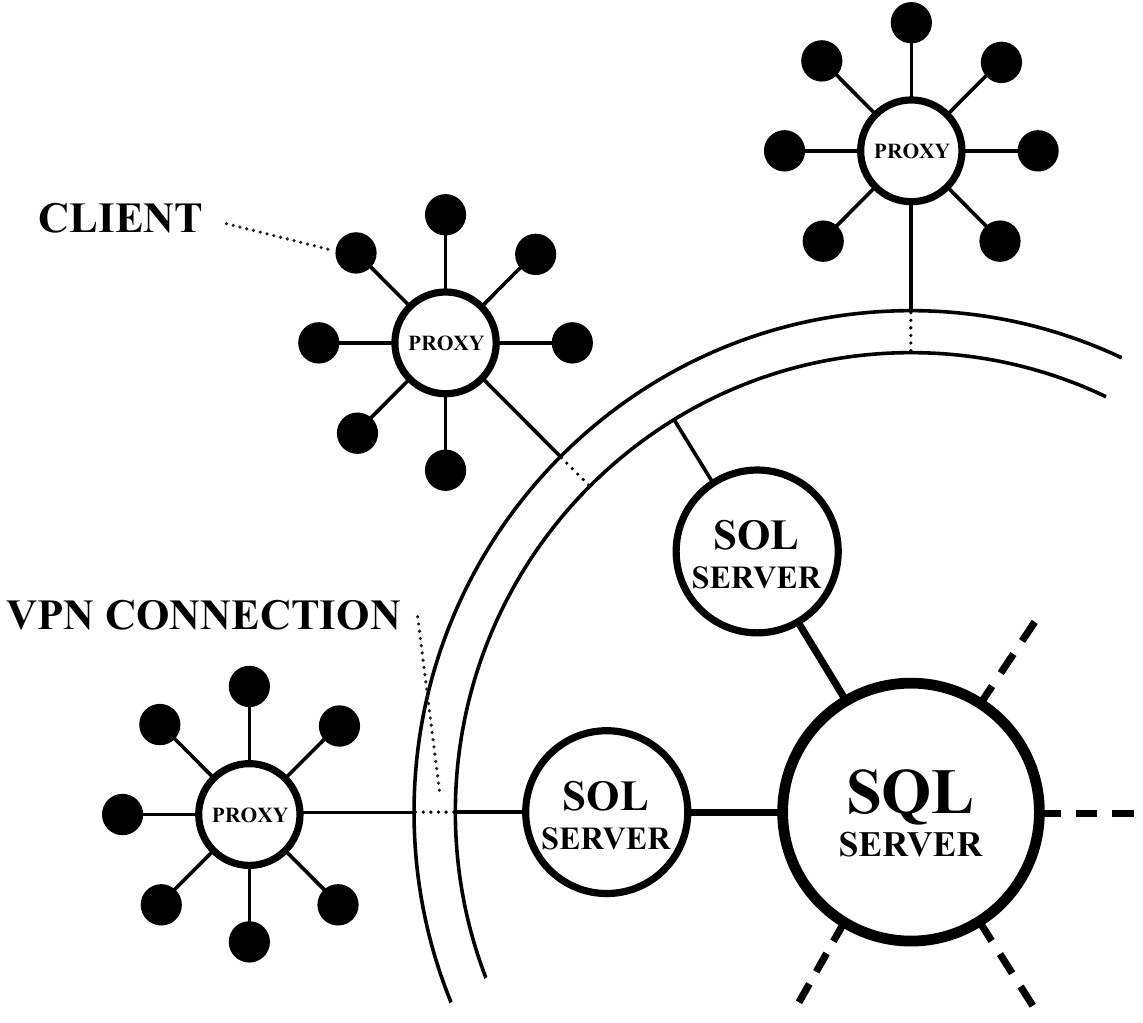
\includegraphics[scale=0.3]{eve.png}
	\end{center}
	\caption{Arquitectura del servidor central de EVE Online}
\end{figure}

\pagebreak

\section{Conclusión}

Los MMORPGs son videojuegos que presentan retos propios de los sistemas distribuidos en cuanto a la experiencia de los jugadores.
Los servidores deben mantener un nivel de latencia aceptablemente bajo y soportar una congregación de jugadores característicamente alta, evitando que éstos puedan realizar ataques al juego en su beneficio.

La forma de afrontar estos retos es propia de cada uno de los juegos, siendo lo normal dividir a los jugadores por regiones, aunque existen juegos que utilizan un único servidor para gestionar las conexiones o que permiten a los jugadores saltar entre los servidores sin necesidad de realizar gestiones especiales.

\begin{thebibliography}{8}
\bibitem{dge_mmosg}
	Cohen, R., Ejlersen, A., Kristensen, R.: Distributed Game Engine for Massively Multiplayer Online Shooting Games (2010). Recuperado de \url{https://www.ejlersen.info/Files/DAT5.pdf} en 4 de abril de 2021

\bibitem{mmg_love}
	Wirt, M.: Massively Multi-player Games and the Systems That Love Them (2005). Recuperado de \url{https://www.usenix.org/legacy/events/usenix05/tech/slides/wirt.pdf} en 4 de abril de 2021

\bibitem{datacomm}
	Larsson, M., Theorén, D.: Datacommunication and Distributed Systems (2005). Recuperado de \url{https://www.cse.chalmers.se/~tsigas/Courses/DCDSeminar/2005/MMORPG.pdf} en 4 de abril de 2021

\bibitem{osrs_servidores}
	Play Old School RuneScape --- World Server List, \url{https://oldschool.runescape.com/slu}. Consultado en 7 de abril de 2021

\bibitem{osrs_bh}
	Bounty Hunter Returns, \url{https://secure.runescape.com/m=news/bounty-hunter-returns?oldschool=1}. Consultado en 7 de abril de 2021

\bibitem{eve_shard}
	Khaleb, K.: Why EVE Online has a single shard server? \url{https://kassiokhaleb.com/eve-online-server}. Consultado en 2 de abril de 2021

\bibitem{inf_space}
	Emilsson, K.: Infinite Space: An Argument for Single-Sharded Architecture in MMOs, \url{https://www.gamasutra.com/view/feature/132563/infinite\_space\_an\_argument\_for\_.php}. Consultado en 2 de abril de 2021

\bibitem{eve_server}
	Drain, B.: EVE Evolved: EVE Online's server model, \url{https://www.engadget.com/2008-09-28-eve-evolved-eve-onlines-server-model.html}. Consultado en 5 de abril de 2021

\bibitem{spython}
	Stackless Python --- Python wiki, \url{https://wiki.python.org/moin/StacklessPython}. Consultado en 5 de abril de 2021
\end{thebibliography}
\end{document}
